\documentclass[11pt,border=2mm,tikz]{standalone}
\usepackage{csquotes}
\usepackage[backend=biber,style=numeric,sorting=none]{biblatex}

\providecommand{\FigScale}{1.1}

\usepackage{siunitx}
\usepackage{tikz}
\usetikzlibrary{calc, positioning, arrows.meta}

\usepackage{amsmath}

\usepackage[siunitx,american]{circuitikz}

\begin{document}
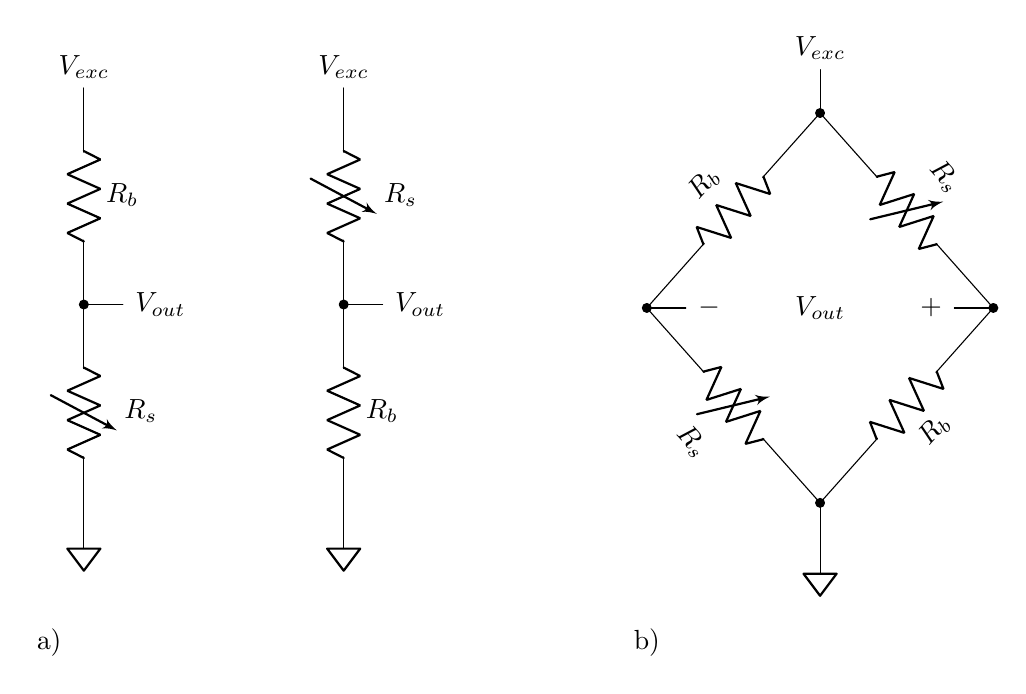
\begin{tikzpicture}[scale=\FigScale, line cap=round, line join=round]


\begin{scope}[shift={(3,0)}]
	\draw (0,5) node[above]{$V_{exc}$}
		to[vR, l=$R_s$] (0,2.5)
		node[circ]{} (0,2.5) -- ++(0.45,0) node[right=1pt]{$V_{out}$} (0,2.5)
		to[R, l=$R_b$] (0,0)
		node[sground]{};
\end{scope}

\begin{scope}
	\draw (0,5) node[above]{$V_{exc}$}
		to[R, l=$R_b$] (0,2.5)
		node[circ]{} (0,2.5) -- ++(0.45,0) node[right=1pt]{$V_{out}$} (0,2.5)
		to[vR, l=$R_s$] (0,0)
		node[sground]{};
\end{scope}

\node at (-0.4,-1.4) {a)};



\begin{scope}[shift={(8.5,0.21)}]
	\coordinate (T) at (0,4.5);
	\coordinate (L) at (-2,2.25);
	\coordinate (R) at (2,2.25);
	\coordinate (B) at (0,0);

	\draw (T) to[short] ++(0,0.5) node[above]{$V_{exc}$};
	\draw (T) to[R, l_=$R_b$] (L);
	\draw (T) to[vR, l=$R_s$] (R);
	\draw (L) to[vR, l_=$R_s$] (B);
	\draw (R) to[R, l=$R_b$] (B);

	\draw (B) to[short] ++(0,-0.5) node[sground]{};

	\node[circ] at (T) {};
	\node[circ] at (L) {};
	\node[circ] at (R) {};
	\node[circ] at (B) {};

	\draw (L) -- ++(0.45,0) node[right=1pt]{$-$};
	\draw (R) -- ++(-0.45,0) node[left=1pt]{$+$};
	\node at (0,2.25) {$V_{out}$};

	\node at (-2,-1.61) {b)};
\end{scope}

\end{tikzpicture}
\end{document}
